% Overleaf has some problems with latexbangla packages : https://tex.stackexchange.com/q/575777/114006
% Download the project and compile it locally. I have complied it perfectly on Miktex latest version.
% !TEX program = xelatex
% !BIB program = biblatex
\documentclass[12pt, oneside]{book}
\usepackage{bookstyle}

\begin{document}

\frontmatter

\title{
\includegraphics[width=0.3\textwidth]{example-image}~\\[0.5cm]
নিবন্ধ সংকলন}
\author{\footnotesize{সম্পাদনায়} \\ 
সম্পাদক\\ 
সহ-সম্পাদক}

\date{\small ২০২১}

\begin{titlepage}

\includepdf[pages=1, fitpaper]{cover}
\thispagestyle{empty}
\predate{\centering \footnotesize{প্রকাশনায়}\\ \large{\href{<url>}{প্রকাশক}} \\}
\postdate{\vfill\hfill \footnotesize{\\অলংকরণে\\ মুবতাসিম ফুয়াদ\\  \uccoff{\fontfamily{lmr}\selectfont ©} \href{https://github.com/rafisics/ebook-template}{আদীব হাসানের টেমপ্লেট}\\}\hfill}     % https://tex.stackexchange.com/a/199356/114006
\maketitle
\end{titlepage}

% Adding dedication and preface                     https://tex.stackexchange.com/a/51539/114006

\pagestyle{empty}
\vspace*{\stretch{1}}
\begin{flushright}
\itshape
আমাদের \\ প্রত্যেক পাঠক এবং শুভাকাঙ্ক্ষীর \\ প্রতি উৎসর্গীকৃত
\end{flushright}
\vspace{\stretch{3}}

\cleardoublepage

\newpage
\pagestyle{plain}
\pagenumbering{roman}

\chapter{সম্পাদকীয়}

		\chapquote{\qtext{One glance at a book and you hear the voice of another person, perhaps someone dead for 1000 years. To read is to voyage through time.}}{কার্ল সেগান}

		\firstword{T}{he} is the preface/abstract of the book.
		\blindtext \\

		\section*{কৃতজ্ঞতা}
		\firstword{T}{he} is the acknowledgement of the book.
		\blindtext \\

		\begin{flushright}
		\itshape
		সম্পাদক, \href{<url>}{নিবন্ধ সংকলন} \\ জুন ২০২১
		\end{flushright}

\cleardoublepage

\setcounter{tocdepth}{0}
\tableofcontents

\newpage
\pagestyle{plain}
\pagenumbering{arabic}

\mainmatter

%article 1   ------------- edit its names as necessary 
\chapter[সূচিপত্রে ১ম নিবন্ধ শিরোনাম]{                                           									% Short chapter title to show on the table of contents
\chapterphoto{example-image-golden}      									                                % Chapter title photo or feature photo
১ম নিবন্ধের পূর্ণ শিরোনাম}                                                               			                    % Full chapter title to show on the chapter title page 
\chapterauthor{\href{https://github.com/rafisics/ebook-template}{১ম নিবন্ধের লেখক}}   % Chapter author name with url 
\newpage
% !TEX program = xelatex
% !BIB program = biblatex
\documentclass[12pt]{article}
% -------------------------------------- The below preambles are only necessary when you try to compile the article invididually.

\usepackage{../articlestyle}

% -------------------------------------- The above preambles are only necessary when you try to compile the article invididually.

\begin{document}

% \begin{figure}[t]
%         \centering
%         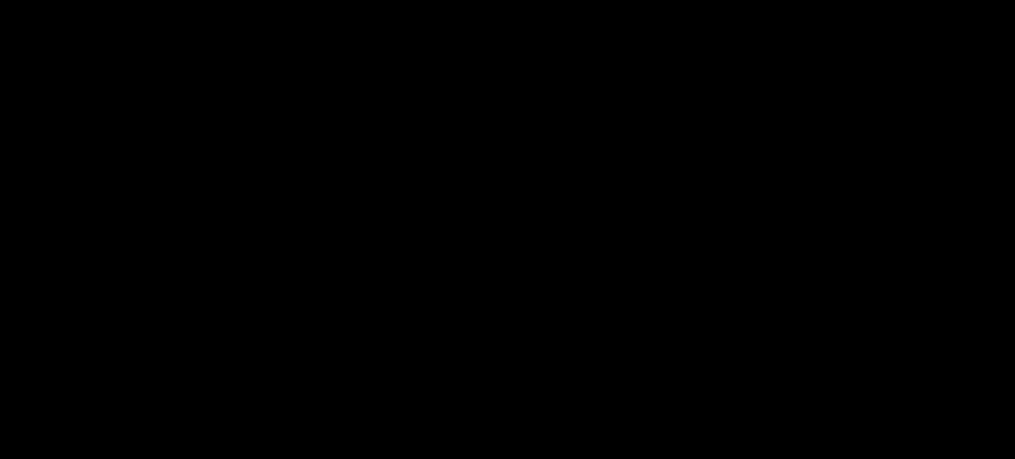
\includegraphics[width=\textwidth]{article1/image.png}
% \end{figure}

\title{১ম নিবন্ধের শিরোনাম}
\author{\href{https://github.com/rafisics/ebook-template}{১ম নিবন্ধের লেখক}}
\date{}

% \maketitle                                % Use \maketitle if you want to compile it individually

\section{সেকশন}

\begin{figure}[hbt!]
        \centering
        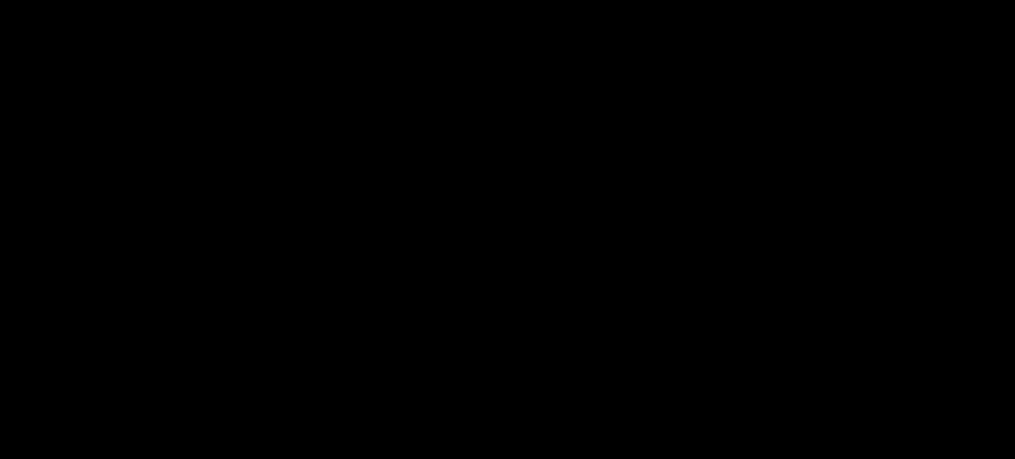
\includegraphics[width=\textwidth]{article1/image.png}
        \caption{Donec vehicula augue eu neque.}
\end{figure}

\firstword{Y}{ou} can put a drop-cap on the first word.
\lipsum

\begin{figure}[hbt!]
    \centering
    \begin{subfigure}[t]{0.5\textwidth}
        \centering
        \includegraphics[height=1.2in]{example-image-a}
        \caption{Image of A}
    \end{subfigure}%
    ~
    \begin{subfigure}[t]{0.5\textwidth}
        \centering
        \includegraphics[height=1.2in]{example-image-b}
        \caption{Image of B}
    \end{subfigure}
    \caption{Comparison between the images of A and B}
\end{figure}

% % generates a paragraph of dummy lorem ipsum text
%\blindtext

% generates multiple paragraphs of dummy lorem ipsum text
% \Blindtext

% % generates whole document with dummy lorem ipsum text
% \Blinddocument

\end{document}
                                             

%article 2   ------------- edit its names as necessary 
\chapter[সূচিপত্রে ২য় নিবন্ধ শিরোনাম]{
\chapterphoto{example-image-golden} 
২য় নিবন্ধের পূর্ণ শিরোনাম}
\chapterauthor{\href{https://github.com/rafisics/ebook-template}{২য় নিবন্ধের লেখক}} 
\newpage
% !TEX program = xelatex
% !BIB program = biblatex
\documentclass[12pt]{article}
% -------------------------------------- The below preambles are only necessary when you try to compile the article invididually.

\usepackage{../articlestyle}

% -------------------------------------- The above preambles are only necessary when you try to compile the article invididually.

\begin{document}

% \begin{figure}[t]
%         \centering
%         \includegraphics[width=\textwidth]{example-image}
% \end{figure}

\title{২য় নিবন্ধের শিরোনাম}
\author{\href{https://github.com/rafisics/ebook-template}{২য় নিবন্ধের লেখক}}
\date{}

% \maketitle                                % Use \maketitle if you want to compile it individually

\begin{figure}[htbp]
        \centering
        \includegraphics[width=0.8\textwidth]{example-image}
        \caption{Donec vehicula augue eu neque.}
\end{figure}

\firstword{Y}{ou} can put a drop-cap on the first word. \blindtext \\

\section*{সেকশন: List Styles}

Using \verb|\begin{itemize} ... \end{itemize}|
\begin{itemize}
        \item Item one
        \item Item two
\end{itemize}

Using \verb|\begin{myitemize} ... \end{myitemize}|
\begin{myitemize}
        \item Item one
        \item Item two
\end{myitemize}

Using \verb|\begin{mylist} ... \end{mylist}|
\begin{mylist}
        \item Item one
        \item Item two
\end{mylist}

Using \verb|\begin{enumerate} ... \end{enumerate}|
\begin{enumerate}
        \item Item one
        \item Item two
\end{enumerate}    

\lipsum[3][1-6]

\section*{সেকশন: Quote Styles}

Example 1. \verb|\chapquote{Quote}[Author][source]|
\chapquote{Lorem ipsum dolor sit amet, consectetur adipiscing elit.}[Quote Author][Quote Source]

Example 2. \verb|\chapquote{Quote}[Author][]|
\chapquote{Lorem ipsum dolor sit amet, consectetur adipiscing elit.}[Quote Author][]    

Example 3. \verb|\chapquote{Quote}[][source]|
\chapquote{Lorem ipsum dolor sit amet, consectetur adipiscing elit.}[][Quote Source]    

Example 4. \verb|\chapquote{Quote}| 
\chapquote{Lorem ipsum dolor sit amet, consectetur adipiscing elit.}

Example 5. \verb|\quote{Quote}| 
\quote{Lorem ipsum dolor sit amet, consectetur adipiscing elit.}

% \lipsum[3][1-6]

% % generates a paragraph of dummy lorem ipsum text
% \blindtext

% generates multiple paragraphs of dummy lorem ipsum text
% \Blindtext

% % generates whole document with dummy lorem ipsum text
% \Blinddocument

\end{document}


% More articles can be added here in the similar way

\end{document}